\documentclass[../summary.tex]{subfiles}

\begin{document}
	
	\section{Food security}
	
	\subsection{Study guide}
	
	Students should understand important concepts such as:
	\begin{itemize} 
	\item Food security
	\item Food gap
	\item Land gap
	\item Yield gap
	\item Synthetic versus bio-based fertilizers
	\item Intensive versus extensive farming
	\item Classic breeding technologies versus genetically modified crops
	\item Plant protection products (PPP)
	\item Integrated pest management (IPM)
	\item Sustainable diet
	\item Protein shift
	\item Food waste
	\item Generational renewal
	\end{itemize}
	In addition, students should understand the environmental impact of food production / agriculture (land use, greenhouse gas emission, nutrient emission by synthetic fertilizers), including differences between animal-based versus plant-based foods.
	\\\\
	Finally, students should have insight into solutions to increase food security (increase yields, adopt healthy
	diets, reduce food waste)
	
	\subsection{Food security}
	
	Food security exists when all people, at all times, have physical and economic access to sufficient, safe and nutritious food that meets their dietary needs and food preferences for an active and healthy life. 
	
	\todo[inline]{Add part about food security }
	
	\subsection{Socio-economic characteristics}
	
	Two particularly important aspects to discuss whether or not we will we be able to produce enough food to feed the world population are the growing world population and the global surface area that can be allocated for food production. 
	\\\\
	The \textbf{food gap} measures how much food is needed to raise consumption at every income level to meet the minimum nutritional intake target per capita per day. Given the current population growth, we can expect a food gap of 56\% by 2050. In other words, where we needed about 13000 trillion calories to feed the world in 2010, we will need to produce over 20000 trillion calories by 2050. This is visualised on Figure \ref{fig:food_gap}.
	\\\\
	
	\begin{figure}[htbp]
	\centering
	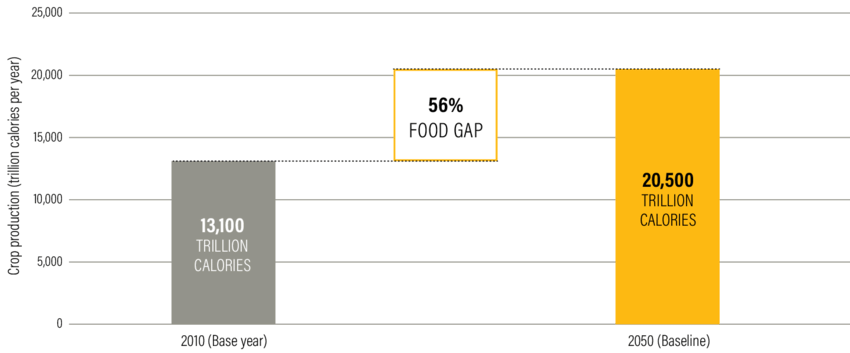
\includegraphics[width=1\linewidth]{images/6-food-gap.png}
	\caption{Food gap}
	\label{fig:food_gap}
	\end{figure}
	
	This food gap is also reflected in the \textbf{land gap}, which is the difference between the projected area of land needed to produce enough food in 2050 and the amount of agricultural land in 2010. On the left of Figure \ref{fig:land_gap}, we can see that we need approximately 600 M ha of land extra to fill the food gap by 2050. This “business-as-usual scenario” considers the past trends in productivity gains we still have for our crop production system worldwide. However, in a second scenario where no productivity gains are taken into account, we need an extra 3200M ha of agricultural land, this is more than 3 times the surface of the United States of America or almost all the land that is now covered by forests.
	\\\\
	\begin{figure}[htbp]
		\centering
		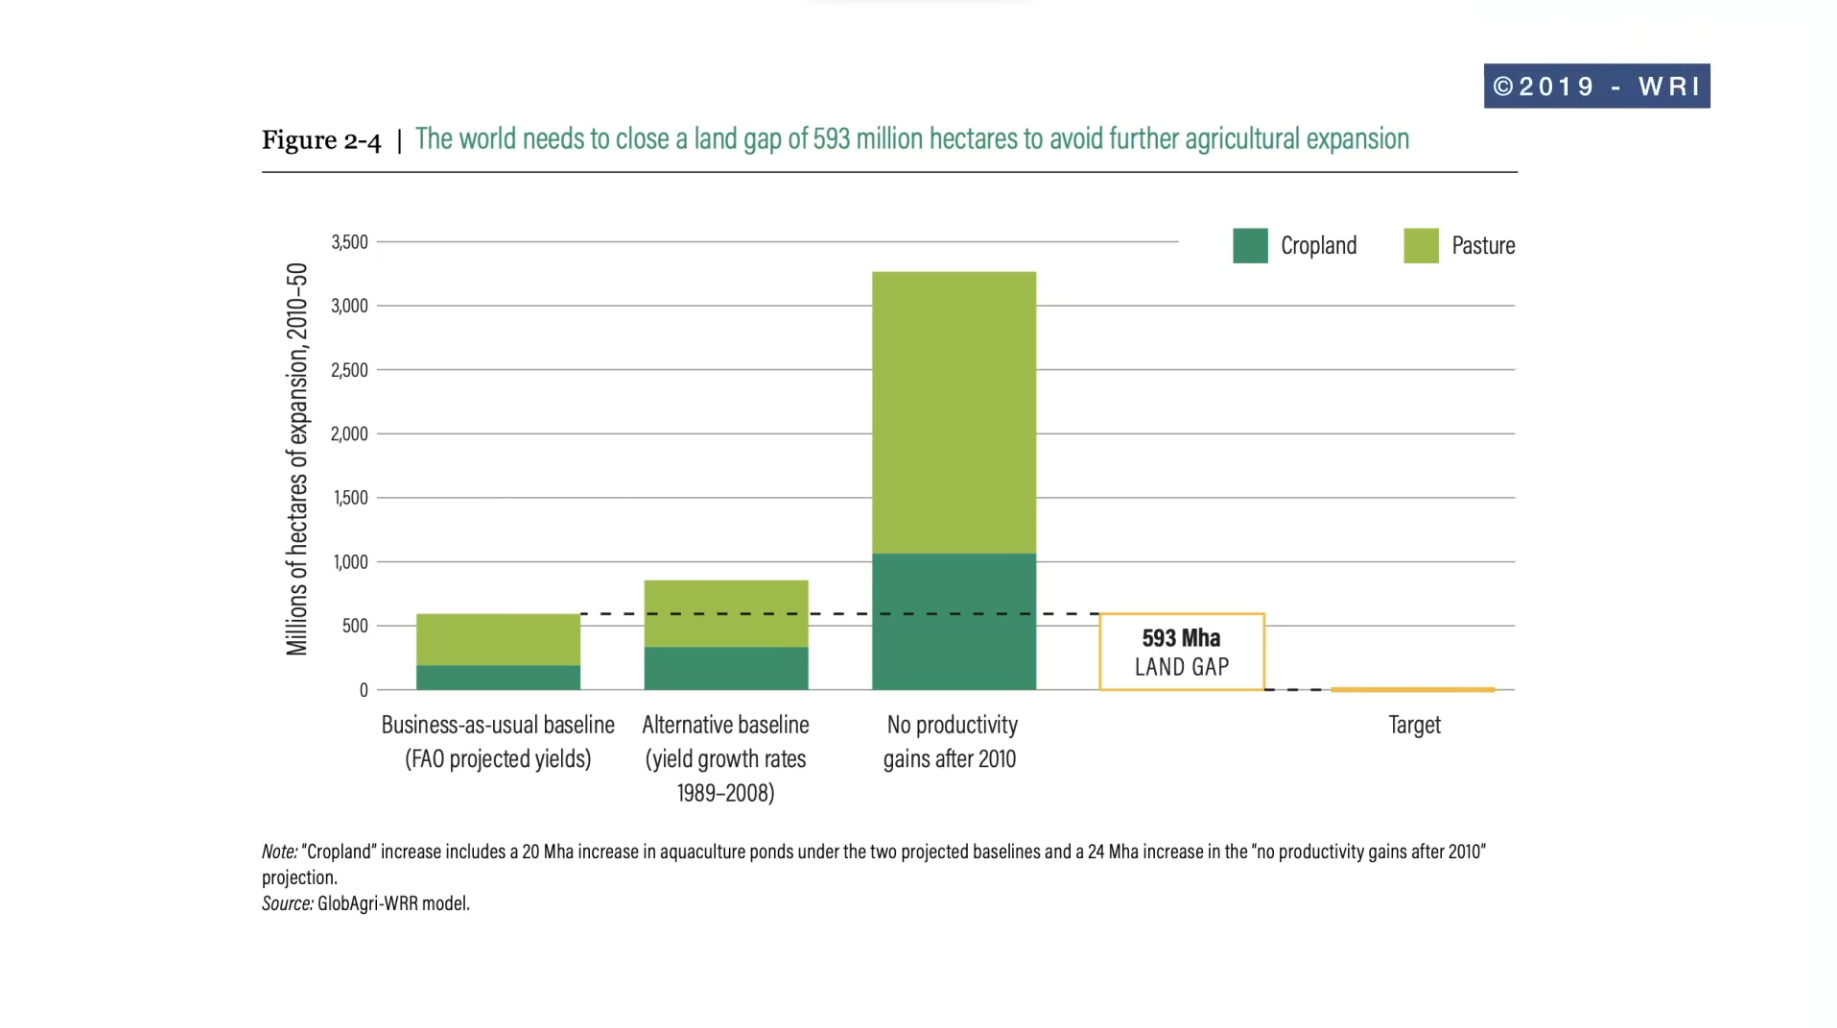
\includegraphics[width=1\linewidth]{images/6-land-gap.png}
		\caption{Land gap}
		\label{fig:land_gap}
	\end{figure}
	
	The yield gap represents the difference between the potential yield that could be achieved with optimal crop management practices and the actual yield obtained by farmers. This gap highlights the untapped potential for increasing production. Factors contributing to the yield gap include limited access to improved seeds, inadequate use of fertilizers and irrigation, pests and diseases and suboptimal agronomic practices. Addressing the yield gap requires targeted interventions, such as improving agricultural infrastructure, providing farmers with access to modern technologies and knowledge, promoting sustainable farming practices and supporting research and development efforts to develop high-yielding and resilient cereal varieties. By narrowing the yield gap, we can enhance global food security and contribute to the sustainable development of agriculture.
	
	\subsection{Environmental impact of agriculture}
	
	\subsection{Sustainable food consumption}
	
\end{document}